\documentclass[a4paper]{article}
%\VignetteIndexEntry{UP - unequal probability sampling designs}
%\VignettePackage{sampling}
\newcommand{\sampling}{{\tt sampling}}
\newcommand{\R}{{\tt R}}
\setlength{\parindent}{0in}
\setlength{\parskip}{.1in}
\setlength{\textwidth}{140mm}
\setlength{\oddsidemargin}{10mm}
\title{Unequal probability sampling designs}
\author{}
\usepackage{Sweave} 

\begin{document}
\maketitle

This is an example of unequal probability (UP) sampling functions (selection of samples using the Belgian municipalities 
data set, with equal or unequal probabilities, and comparison of the accuracy of the Horvitz-Thompson estimator by boxplots).                                                 
The used sampling schemes are: Poisson, random systematic, random pivotal, Till\'e, Midzuno, systematic, 
pivotal, and simple random sampling without replacement. 

\begin{Schunk}
\begin{Sinput}
> b = data(belgianmunicipalities)
> pik = inclusionprobabilities(belgianmunicipalities$Tot04, 
+     200)
> N = length(pik)
> n = sum(pik)
\end{Sinput}
\end{Schunk}
Number of simulations (for an accurate result, increase this value):

\begin{Schunk}
\begin{Sinput}
> sim = 10
> ss = array(0, c(sim, 8))
\end{Sinput}
\end{Schunk}
Defines the interest variable:

\begin{Schunk}
\begin{Sinput}
> y = belgianmunicipalities$TaxableIncome
\end{Sinput}
\end{Schunk}
Simulation and computation of the Horvitz-Thompson estimator:

\begin{Schunk}
\begin{Sinput}
> ht = numeric(8)
> for (i in 1:sim) {
+     cat("Step ", i, "\n")
+     s = UPpoisson(pik)
+     ht[1] = HTestimator(y[s == 1], pik[s == 1])
+     s = UPrandomsystematic(pik)
+     ht[2] = HTestimator(y[s == 1], pik[s == 1])
+     s = UPrandompivotal(pik)
+     ht[3] = HTestimator(y[s == 1], pik[s == 1])
+     s = UPtille(pik)
+     ht[4] = HTestimator(y[s == 1], pik[s == 1])
+     s = UPmidzuno(pik)
+     ht[5] = HTestimator(y[s == 1], pik[s == 1])
+     s = UPsystematic(pik)
+     ht[6] = HTestimator(y[s == 1], pik[s == 1])
+     s = UPpivotal(pik)
+     ht[7] = HTestimator(y[s == 1], pik[s == 1])
+     s = srswor(n, N)
+     ht[8] = HTestimator(y[s == 1], rep(n/N, n))
+     ss[i, ] = ss[i, ] + ht
+ }
\end{Sinput}
\end{Schunk}
Boxplots of the estimators:

\begin{Schunk}
\begin{Sinput}
> colnames(ss) <- c("poisson", "rsyst", "rpivotal", 
+     "tille", "midzuno", "syst", "pivotal", "srswor")
> boxplot(data.frame(ss), las = 3)
\end{Sinput}
\end{Schunk}
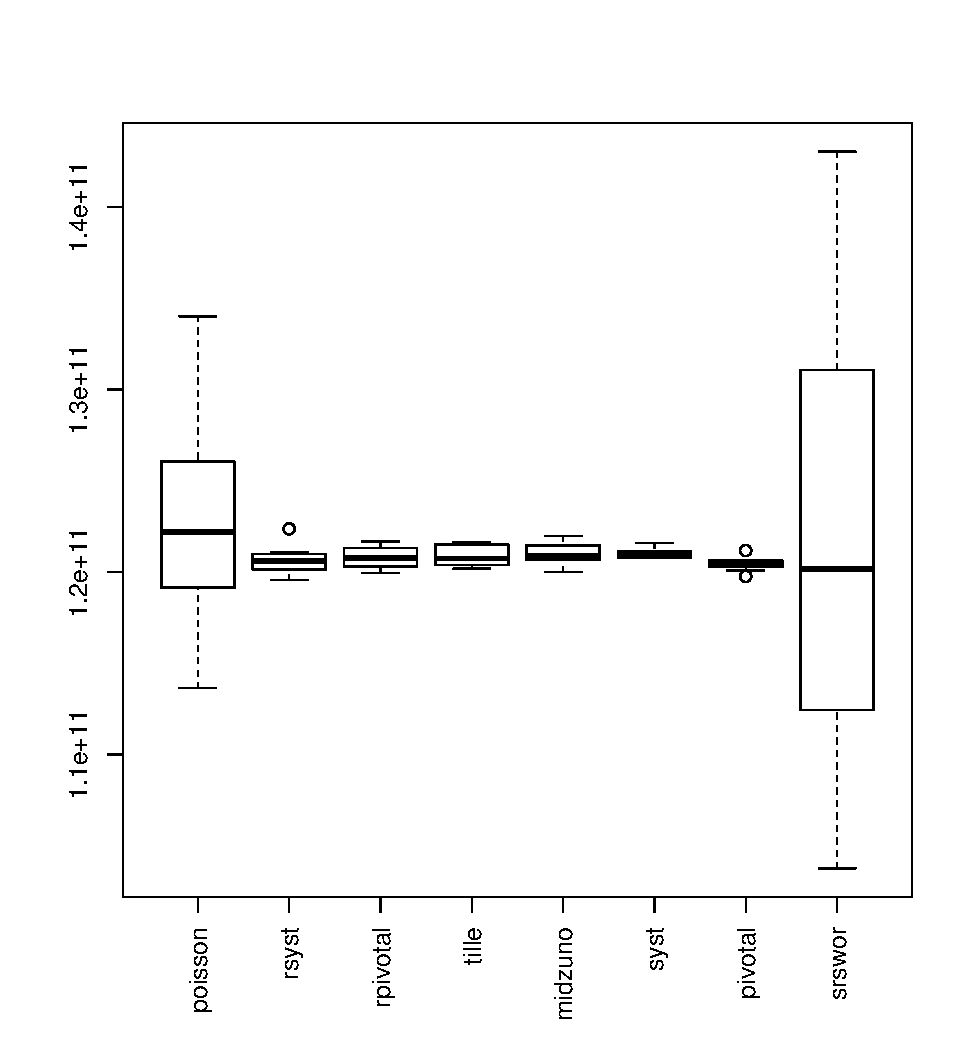
\includegraphics{UPexamples-up5}
\end{document}

